\documentclass[14pt]{extbook}
\usepackage{multicol, enumerate, enumitem, hyperref, color, soul, setspace, parskip, fancyhdr} %General Packages
\usepackage{amssymb, amsthm, amsmath, bbm, latexsym, units, mathtools} %Math Packages
\everymath{\displaystyle} %All math in Display Style
% Packages with additional options
\usepackage[headsep=0.5cm,headheight=12pt, left=1 in,right= 1 in,top= 1 in,bottom= 1 in]{geometry}
\usepackage[usenames,dvipsnames]{xcolor}
\usepackage{dashrule}  % Package to use the command below to create lines between items
\newcommand{\litem}[1]{\item#1\hspace*{-1cm}\rule{\textwidth}{0.4pt}}
\pagestyle{fancy}
\lhead{Progress Quiz 4}
\chead{}
\rhead{Version C}
\lfoot{6286-1986}
\cfoot{}
\rfoot{Fall 2020}
\begin{document}

\begin{enumerate}
\litem{
Describe the end behavior of the polynomial below.\[ f(x) = -3(x - 8)^{2}(x + 8)^{5}(x + 9)^{3}(x - 9)^{3} \]\begin{enumerate}[label=\Alph*.]
\begin{multicols}{2}\item 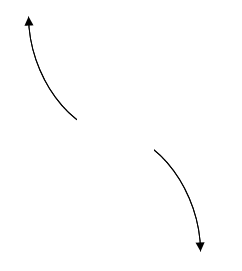
\includegraphics[width = 0.3\textwidth]{../Figures/polyEndBehaviorCopyAC.png}\item 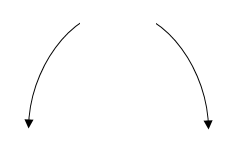
\includegraphics[width = 0.3\textwidth]{../Figures/polyEndBehaviorCopyBC.png}\item 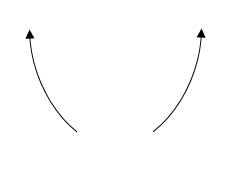
\includegraphics[width = 0.3\textwidth]{../Figures/polyEndBehaviorCopyCC.png}\item 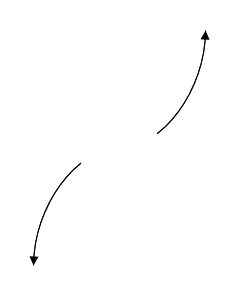
\includegraphics[width = 0.3\textwidth]{../Figures/polyEndBehaviorCopyDC.png}\end{multicols}\item None of the above.
\end{enumerate} }
\litem{
Construct the lowest-degree polynomial given the zeros below. Then, choose the intervals that contain the coefficients of the polynomial in the form $ax^3+bx^2+cx+d$.\[ \frac{7}{3}, \frac{-2}{5}, \text{ and } \frac{5}{3} \]\begin{enumerate}[label=\Alph*.]
\item \( a \in [40, 47], b \in [157, 164], c \in [98, 105], \text{ and } d \in [-78, -62] \)
\item \( a \in [40, 47], b \in [10, 18], c \in [-187, -180], \text{ and } d \in [67, 80] \)
\item \( a \in [40, 47], b \in [44, 51], c \in [-164, -157], \text{ and } d \in [-78, -62] \)
\item \( a \in [40, 47], b \in [-162, -159], c \in [98, 105], \text{ and } d \in [67, 80] \)
\item \( a \in [40, 47], b \in [-162, -159], c \in [98, 105], \text{ and } d \in [-78, -62] \)

\end{enumerate} }
\litem{
Construct the lowest-degree polynomial given the zeros below. Then, choose the intervals that contain the coefficients of the polynomial in the form $x^3+bx^2+cx+d$.\[ 5 + 3 i \text{ and } 1 \]\begin{enumerate}[label=\Alph*.]
\item \( b \in [-5, 2], c \in [-4, -1], \text{ and } d \in [2.3, 3.8] \)
\item \( b \in [-21, -10], c \in [43, 45], \text{ and } d \in [-36.5, -33.9] \)
\item \( b \in [9, 16], c \in [43, 45], \text{ and } d \in [33.9, 36.3] \)
\item \( b \in [-5, 2], c \in [-9, -5], \text{ and } d \in [4.4, 5.8] \)
\item \( \text{None of the above.} \)

\end{enumerate} }
\litem{
Describe the end behavior of the polynomial below.\[ f(x) = 2(x + 7)^{3}(x - 7)^{4}(x - 3)^{4}(x + 3)^{6} \]\begin{enumerate}[label=\Alph*.]
\begin{multicols}{2}\item 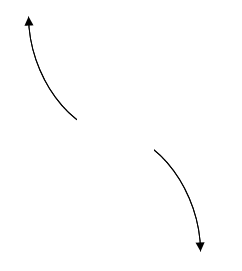
\includegraphics[width = 0.3\textwidth]{../Figures/polyEndBehaviorAC.png}\item 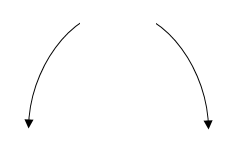
\includegraphics[width = 0.3\textwidth]{../Figures/polyEndBehaviorBC.png}\item 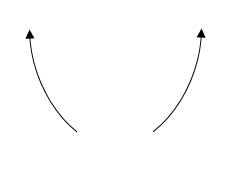
\includegraphics[width = 0.3\textwidth]{../Figures/polyEndBehaviorCC.png}\item 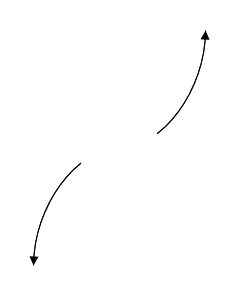
\includegraphics[width = 0.3\textwidth]{../Figures/polyEndBehaviorDC.png}\end{multicols}\item None of the above.
\end{enumerate} }
\litem{
Which of the following equations \textit{could} be of the graph presented below?
\begin{center}
    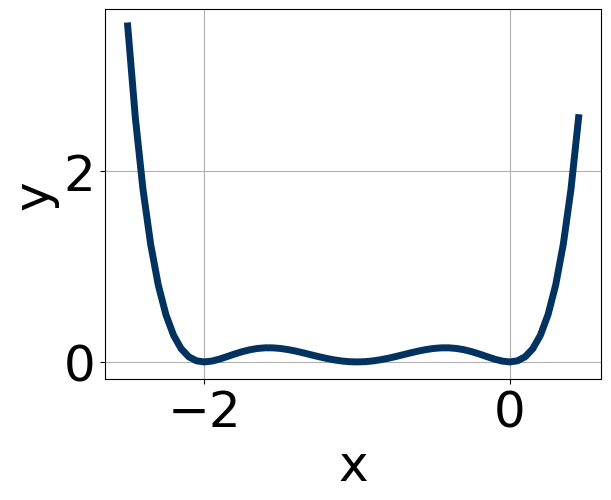
\includegraphics[width=0.5\textwidth]{../Figures/polyGraphToFunctionCopyC.png}
\end{center}
\begin{enumerate}[label=\Alph*.]
\item \( -14(x - 2)^{6} (x + 2)^{8} (x - 3)^{6} \)
\item \( 20(x - 2)^{10} (x + 2)^{8} (x - 3)^{6} \)
\item \( -5(x - 2)^{10} (x + 2)^{10} (x - 3)^{5} \)
\item \( 4(x - 2)^{8} (x + 2)^{6} (x - 3)^{5} \)
\item \( 9(x - 2)^{8} (x + 2)^{11} (x - 3)^{5} \)

\end{enumerate} }
\litem{
Which of the following equations \textit{could} be of the graph presented below?
\begin{center}
    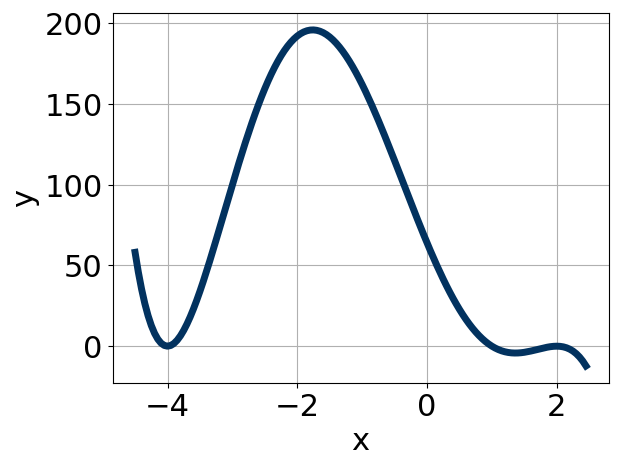
\includegraphics[width=0.5\textwidth]{../Figures/polyGraphToFunctionC.png}
\end{center}
\begin{enumerate}[label=\Alph*.]
\item \( 6x^{4} (x - 3)^{10} (x + 1)^{4} \)
\item \( 9x^{10} (x - 3)^{6} (x + 1)^{11} \)
\item \( -5x^{8} (x - 3)^{8} (x + 1)^{9} \)
\item \( -19x^{7} (x - 3)^{6} (x + 1)^{6} \)
\item \( -10x^{11} (x - 3)^{4} (x + 1)^{9} \)

\end{enumerate} }
\litem{
Construct the lowest-degree polynomial given the zeros below. Then, choose the intervals that contain the coefficients of the polynomial in the form $ax^3+bx^2+cx+d$.\[ \frac{-7}{5}, 5, \text{ and } 2 \]\begin{enumerate}[label=\Alph*.]
\item \( a \in [4, 9], b \in [-45, -40], c \in [95, 103], \text{ and } d \in [-73, -67] \)
\item \( a \in [4, 9], b \in [22, 34], c \in [-8, 8], \text{ and } d \in [-73, -67] \)
\item \( a \in [4, 9], b \in [-34, -27], c \in [-8, 8], \text{ and } d \in [70, 73] \)
\item \( a \in [4, 9], b \in [5, 9], c \in [-74, -67], \text{ and } d \in [70, 73] \)
\item \( a \in [4, 9], b \in [-34, -27], c \in [-8, 8], \text{ and } d \in [-73, -67] \)

\end{enumerate} }
\litem{
Describe the zero behavior of the zero $x = 9$ of the polynomial below.\[ f(x) = 9(x + 9)^{6}(x - 9)^{9}(x - 3)^{5}(x + 3)^{7} \]\begin{enumerate}[label=\Alph*.]
\begin{multicols}{2}\item 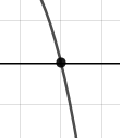
\includegraphics[width = 0.3\textwidth]{../Figures/polyZeroBehaviorCopyAC.png}\item 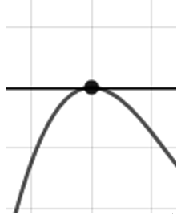
\includegraphics[width = 0.3\textwidth]{../Figures/polyZeroBehaviorCopyBC.png}\item 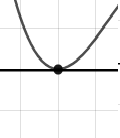
\includegraphics[width = 0.3\textwidth]{../Figures/polyZeroBehaviorCopyCC.png}\item 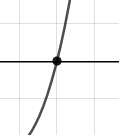
\includegraphics[width = 0.3\textwidth]{../Figures/polyZeroBehaviorCopyDC.png}\end{multicols}\item None of the above.
\end{enumerate} }
\litem{
Construct the lowest-degree polynomial given the zeros below. Then, choose the intervals that contain the coefficients of the polynomial in the form $x^3+bx^2+cx+d$.\[ 2 + 5 i \text{ and } 3 \]\begin{enumerate}[label=\Alph*.]
\item \( b \in [1, 2], c \in [-9.1, -7.3], \text{ and } d \in [10, 22] \)
\item \( b \in [-7, -4], c \in [40.5, 41.2], \text{ and } d \in [-93, -85] \)
\item \( b \in [1, 2], c \in [-5.6, -1.6], \text{ and } d \in [3, 7] \)
\item \( b \in [6, 14], c \in [40.5, 41.2], \text{ and } d \in [87, 89] \)
\item \( \text{None of the above.} \)

\end{enumerate} }
\litem{
Describe the zero behavior of the zero $x = -7$ of the polynomial below.\[ f(x) = 2(x - 9)^{13}(x + 9)^{9}(x - 7)^{7}(x + 7)^{4} \]\begin{enumerate}[label=\Alph*.]
\begin{multicols}{2}\item 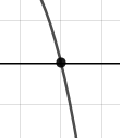
\includegraphics[width = 0.3\textwidth]{../Figures/polyZeroBehaviorAC.png}\item 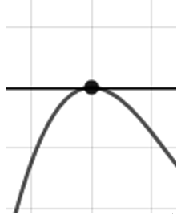
\includegraphics[width = 0.3\textwidth]{../Figures/polyZeroBehaviorBC.png}\item 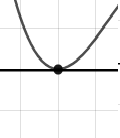
\includegraphics[width = 0.3\textwidth]{../Figures/polyZeroBehaviorCC.png}\item 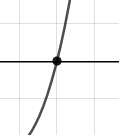
\includegraphics[width = 0.3\textwidth]{../Figures/polyZeroBehaviorDC.png}\end{multicols}\item None of the above.
\end{enumerate} }
\end{enumerate}

\end{document}